% This LaTeX document needs to be compiled with XeLaTeX.
\documentclass[10pt]{article}
\usepackage[utf8]{inputenc}
\usepackage{graphicx}
\usepackage[export]{adjustbox}
\graphicspath{ {./images/} }
\usepackage{amsmath}
\usepackage{amsfonts}
\usepackage{amssymb}
\usepackage[version=4]{mhchem}
\usepackage{stmaryrd}
\usepackage[fallback]{xeCJK}
\usepackage{polyglossia}
\usepackage{fontspec}
\setCJKmainfont{Noto Serif CJK TC}

\setmainlanguage{polish}
\setmainfont{CMU Serif}

\title{Instrukcja dla zdającego }

\author{}
\date{}


\newcommand\Varangle{\mathop{{<\!\!\!\!\!\text{\small)}}\:}\nolimits}

\begin{document}
\maketitle
\begin{center}

\includegraphics[max width=\textwidth]{2024_11_21_23d228cacd5e4a9a3f86g-01}
\end{center}

MATEMATYKA - poziom podstawowy - klasa 1\\
MAJ 2019\\
LSCDN

Czas pracy:

\begin{enumerate}
  \item Sprawdź, czy arkusz zawiera 16 stron.
  \item Rozwiązania zadań i odpowiedzi zamieść w miejscu na to przeznaczonym.
  \item W zadaniach od 1 do 25 są podane 4 odpowiedzi: \(\mathrm{A}, \mathrm{B}, \mathrm{C}, \mathrm{D}\), z których tylko jedna jest prawdziwa. Wybierz tylko jedną odpowiedź i zaznacz ją na karcie odpowiedzi.
  \item Zaznaczając odpowiedzi w części karty przeznaczonej dla zdającego, zamaluj pola do tego przeznaczone. Błędne zaznaczenie otocz kółkiem i zaznacz właściwe.
  \item Rozwiązania zadań od 26 do 34 zapisz starannie i czytelnie w wyznaczonych miejscach. Przedstaw swój tok rozumowania prowadzący do ostatecznego wyniku.
  \item Pamiętaj, że pominięcie argumentacji lub istotnych obliczeń w rozwiązaniu zadania otwartego może spowodować, że za to rozwiązanie możesz nie dostać pełnej liczby punktów.
  \item Pisz czytelnie. Używaj długopisu/pióra tylko z czarnym tuszem/atramentem.
  \item Nie używaj korektora. Błędne zapisy przekreśl.
  \item Pamiętaj, że zapisy w brudnopisie nie podlegają ocenie.
  \item Obok numeru każdego zadania podana jest maksymalna liczba punktów możliwych do uzyskania.
  \item Możesz korzystać z zestawu wzorów matematycznych, cyrkla i linijki oraz kalkulatora.
  \item Wypełnij tę częsć karty odpowiedzi, którą koduje zdający. Nie wpisuj żadnych znaków części przeznaczonej dla egzaminatora.
\end{enumerate}

Liczba\\
punktów\\
do\\
uzyskania:\\
50

\section*{ZADANIA ZAMKNIETE}
W zadaniach o numerach od 1 do 25 wybierz i zaznacz na karcie odpowiedzi jedną poprawną odpowiedź.

Zadanie 1. (1pkt)\\
Wartość wyrażenia \(\frac{1}{2} \log _{5} 81-\frac{1}{2} \log _{5} 36\) jest równa:\\
A. \(\frac{1}{2} \log _{5} 45\)\\
B. \(\log _{5} \frac{3}{2}\)\\
C. \(\log _{5} 3\)\\
D. \(\log _{5} 15\)

\section*{Zadanie 2. (1pkt)}
Liczba \(\frac{4^{\frac{3}{2}} \cdot 36^{-\frac{1}{2}}}{3^{-2}}\) jest równa:\\
A. \(\frac{4}{27}\)\\
B. 8\\
C. 9\\
D. 12

Zadanie 3. (1pkt)\\
Wyrażenie \(\frac{\left(x^{7}\right)^{-3} \cdot\left(\frac{1}{x}\right)^{5}}{\left(x^{-4}\right)^{\frac{3}{2}}}\) jest równe:\\
A. \(x^{-20}\)\\
B. \(x^{22}\)\\
C. \(x^{-32}\)\\
D. \(x^{-10}\)

Zadanie 4. (1pkt)\\
Wartość wyrażenia \(2|1-\sqrt{3}|-|3-2 \sqrt{3}|\) wynosi:\\
A. -1\\
B. \(4 \sqrt{3}-5\)\\
C. 1\\
D. \(4 \sqrt{3}+1\)

\section*{Zadanie 5. (1pkt)}
Liczbą przeciwną do liczby \(\frac{1}{4+2 \sqrt{2}}\) jest:\\
A. \(\frac{1}{4-2 \sqrt{2}}\)\\
B. \(4+2 \sqrt{2}\)\\
C. \(\frac{-2-\sqrt{2}}{4}\)\\
D. \(\frac{\sqrt{2}}{4}-\frac{1}{2}\)

\section*{Zadanie 6. (1pkt)}
Cenę pewnego towaru podniesiono o \(10 \%\), a następnie obniżono o \(15 \%\). Cena po obu zmianach stanowi x\% początkowej ceny towaru. Zatem\\
A. \(x=95\)\\
B. \(x=103,5\)\\
C. \(x=93,5\)\\
D. \(x=126,5\)

\section*{Zadanie 7. (1pkt)}
Do zbioru liczb wymiernych nie należy liczba:\\
A. \(4^{\frac{3}{2}}\)\\
B. \(4^{\frac{1}{8}}: 4^{-\frac{3}{8}}\)\\
C. \(\left(4^{\frac{7}{4}}\right)^{-2}\)\\
D. \(4^{\frac{3}{4}} \cdot 4^{\frac{1}{2}}\)

\section*{Zadanie 8. (1pkt)}
Jeżeli \(a=\log _{\frac{1}{3}} 9\) oraz \(b=\log _{36} \frac{1}{6}\), to:\\
A. \(a=4 b\)\\
B. \(a>b\)\\
C. \(a=b\)\\
D. \(b=2 a\)

Zadanie 9. (1pkt)\\
Ułamek \(\frac{9}{11}\) przybliżono z dokładnością do 0,01 . Błąd względny tego przybliżenia wynosi:\\
A. \(\frac{1}{100}\)\\
B. \(\frac{1}{450}\)\\
C. \(\frac{9}{1100}\)\\
D. \(\frac{1}{550}\)

Zadanie 10. (1pkt)\\
Wyrażenie \((x+3 y)^{2}-(3 x-y)^{2}\) jest równe:\\
A. \(-8 x^{2}+10 y^{2}\)\\
B. \(10\left(x^{2}+y^{2}\right)\)\\
C. \(8\left(y^{2}-x^{2}\right)\)\\
D. \(8 y^{2}+12 x y-8 x^{2}\)

Zadanie 11. (1pkt)\\
Dane są zbiory: \(A=\langle-2 ; 1)\) oraz \(B=(-4 ; 9\rangle\). Różnica \(B \backslash A\) jest równa:\\
A. \(\varnothing\)\\
B. \((-4 ;-2\rangle \cup(1 ; 9\rangle\)\\
C. \((-4 ;-2) \cup\langle 1 ; 9\rangle\)\\
D. \((-4 ;-2)\)

Zadanie 12. (1pkt)\\
Rozwiązaniami równania \(\frac{\left(x^{2}-4\right)(x+1)}{\left(x^{2}-1\right)(x+2)}=0\) są liczby:\\
A. 2\\
B. \(-2 ;-1 ; 2\)\\
C. \(-2 ;-1 ; 1 ; 2\)\\
D. \(1 ; 2\)

Zadanie 13. (1pkt)\\
Układ równań \(\left\{\begin{array}{c}5 x+(a+1) y=3 \\ -x+2 y=a+2\end{array}\right.\) jest sprzeczny dla \(a\) równego:\\
A. -11\\
B. 9\\
C. 4\\
D. -1

Zadanie 14. (1pkt)\\
Do zbioru rozwiązań nierówności \(2(x-3)-3(5+x)>9\) należy liczba:\\
A. 30\\
B. -31\\
C. -29\\
D. -30

Zadanie 15. (1pkt)\\
Dziedziną funkcji \(f(x)=\sqrt{21-5 x}\) jest zbiór:\\
A. \(\left(4 \frac{1}{5} ;+\infty\right)\)\\
B. \(\left(-\infty ; 4 \frac{1}{5}\right)\)\\
C. \(\left(-\infty ; 4 \frac{1}{5}\right)\)\\
D. \(\left(4 \frac{1}{5} ;+\infty\right)\)

Zadanie 16. (1pkt)\\
Funkcja \(f(x)=-(2 m-3) x+m-5\) przyjmuje wartość -2 dla argumentu równego -1 . Zatem:\\
A. \(m=-\frac{2}{5}\)\\
B. \(m=2\)\\
C. \(m=0\)\\
D. \(m=\frac{2}{3}\)

\section*{Zadanie 17. (1pkt)}
Wartość wyrażenia \(2 \cos 120^{\circ}+\operatorname{tg} 135^{\circ}\) jest równa:\\
A. 2\\
B. \(\sqrt{3}+1\)\\
C. \(-\sqrt{3}-1\)\\
D. -2

Zadanie 18. (1pkt)\\
Jedna z przyprostokątnych w trójkącie prostokątnym ma długość 3 cm , a przeciwprostokątna 4 cm . Najmniejszym kątem tego trójkąta jest \(\alpha\). Wartość wyrażenia \(\sin ^{2} \alpha-\cos \alpha\) wynosi:\\
A. \(\frac{\sqrt{7}-3}{4}\)\\
B. \(-\frac{5}{16}\)\\
C. \(\frac{9-\sqrt{7}}{16}\)\\
D. 1

\section*{Zadanie 19.}
Jeden z kątów ostrych trójkąta prostokątnego ma miarę \(30^{\circ}\). Dłuższa przyprostokątna tego trójkąta ma długość 6 cm . Promień okręgu opisanego na tym trójkącie ma długość:\\
A. \(2 \sqrt{3}\)\\
B. 6\\
C. \(\frac{3 \sqrt{3}}{2}\)\\
D. \(4 \sqrt{3}\)

Zadanie 20. (1pkt)\\
Punkt S jest środkiem okręgu (rysunek).\\
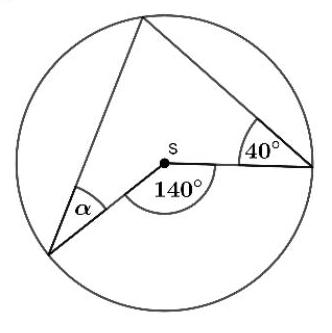
\includegraphics[max width=\textwidth, center]{2024_11_21_23d228cacd5e4a9a3f86g-06(1)}

Miara kąta \(\alpha\) wynosi:\\
A. \(30^{\circ}\)\\
B. \(40^{\circ}\)\\
C. \(70^{\circ}\)\\
D. \(20^{\circ}\)

Zadanie 21. (1pkt)\\
Obwód trójkąta prostokątnego równoramiennego wynosi \(4(1+\sqrt{2})\). Długość wysokości poprowadzonej z wierzchołka kąta prostego tego trójkąta jest równa:\\
A. \(\sqrt{2}\)\\
B. 4\\
C. 2\\
D. \(2 \sqrt{2}\)

Zadanie 22. (1pkt)\\
Punkty A, B, D leżą na jednej prostej. Odcinek AB jest podstawą trójkąta równoramiennego ABC (rysunek).\\
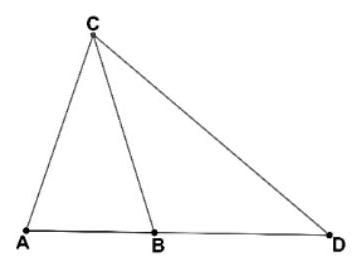
\includegraphics[max width=\textwidth, center]{2024_11_21_23d228cacd5e4a9a3f86g-06}

Jeżeli \(|\Varangle C B D|=3 \cdot|\Varangle A C B|\), to \(|\Varangle D A C|\) wynosi:\\
A. \(108^{\circ}\)\\
B. \(72^{\circ}\)\\
C. \(36^{\circ}\)\\
D. \(54^{\circ}\)

\section*{Zadanie 23. (1pkt)}
Najkrótszy bok trójkąta prostokątnego ma długość 5 cm , a najdłuższy 13 cm . Pole tego trójkąta jest równe:\\
A. \(60 \mathrm{~cm}^{2}\)\\
B. \(65 \mathrm{~cm}^{2}\)\\
C. \(30 \mathrm{~cm}^{2}\)\\
D. \(78 \mathrm{~cm}^{2}\)

\section*{Zadanie 24. (1pkt)}
Ramię trójkąta równoramiennego ABC ma długość 8 , a jeden z kątów tego trójkąta ma miarę \(135^{\circ}\). Pole tego trójkąta jest równe\\
A. \(32 \sqrt{2}\)\\
B. \(16 \sqrt{3}\)\\
C. 32\\
D. \(16 \sqrt{2}\)

Zadanie 25. (1pkt)\\
Trójkąt ACE jest prostokątny oraz \(A E \| B D\) (rysunek).\\
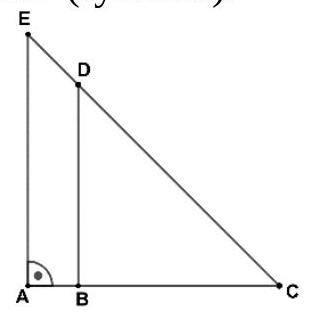
\includegraphics[max width=\textwidth, center]{2024_11_21_23d228cacd5e4a9a3f86g-06(2)}

Jeżeli \(|B D|=\frac{4}{5}|A E|\) oraz \(|B C|=8 \mathrm{~cm}\), to:\\
A. \(|A B|=2 \mathrm{~cm}\)\\
B. \(|A C|=12 \mathrm{~cm}\)\\
C. \(|A B|=4 \mathrm{~cm}\)\\
D. \(|A C|=9 \mathrm{~cm}\)

\section*{ZADANIA OTWARTE}
Rozwiązania zadań o numerach od 26 do 34 należy zapisać w wyznaczonych miejscach pod treścią zadania.\\
Zadanie 26. (2 pkt)\\
Rozwiąż równanie \((x+4)^{2}-2 x^{2}=-(x-6)^{2}\).

\begin{center}
\begin{tabular}{|c|c|c|c|c|c|c|c|c|c|c|c|c|c|c|c|c|c|c|c|c|c|c|c|c|c|c|c|c|c|c|}
\hline
 &  &  &  &  &  &  &  &  &  &  &  &  &  &  &  &  &  &  &  &  &  &  &  &  &  &  &  &  &  &  \\
\hline
 &  &  &  &  &  &  &  &  &  &  &  &  &  &  &  &  &  &  &  &  &  &  &  &  &  &  &  &  &  &  \\
\hline
 &  &  &  &  &  &  &  &  &  &  &  &  &  &  &  &  &  &  &  &  &  &  &  &  &  &  &  &  &  &  \\
\hline
 &  &  &  &  &  &  &  &  &  &  &  &  &  &  &  &  &  &  &  &  &  &  &  &  &  &  &  &  &  &  \\
\hline
 &  &  &  &  &  &  &  &  &  &  &  &  &  &  &  &  &  &  &  &  &  &  &  &  &  &  &  &  &  &  \\
\hline
 &  &  &  &  &  &  &  &  &  &  &  &  &  &  &  &  &  &  &  &  &  &  &  &  &  &  &  &  &  &  \\
\hline
 &  &  &  &  &  &  &  &  &  &  &  &  &  &  &  &  &  &  &  &  &  &  &  &  &  &  &  &  &  &  \\
\hline
 &  &  &  &  &  &  &  &  &  &  &  &  &  &  &  &  &  &  &  &  &  &  &  &  &  &  &  &  &  &  \\
\hline
 &  &  &  &  &  &  &  &  &  &  &  &  &  &  &  &  &  &  &  &  &  &  &  &  &  &  &  &  &  &  \\
\hline
 &  &  &  &  &  &  &  &  &  &  &  &  &  &  &  &  &  &  &  &  &  &  &  &  &  &  &  &  &  &  \\
\hline
 &  &  &  &  &  &  &  &  &  &  &  &  &  &  &  &  &  &  &  &  &  &  &  &  &  &  &  &  &  &  \\
\hline
 &  &  &  &  &  &  &  &  &  &  &  &  &  &  &  &  &  &  &  &  &  &  &  &  &  &  &  &  &  &  \\
\hline
 &  &  &  &  &  &  &  &  &  &  &  &  &  &  &  &  &  &  &  &  &  &  &  &  &  &  &  &  &  &  \\
\hline
 &  &  &  &  &  &  &  &  &  &  &  &  &  &  &  &  &  &  &  &  &  &  &  &  &  &  &  &  &  &  \\
\hline
 &  &  &  &  &  &  &  &  &  &  &  &  &  &  &  &  &  &  &  &  &  &  &  &  &  &  &  &  &  &  \\
\hline
 &  &  &  &  &  &  &  &  &  &  &  &  &  &  &  &  &  &  &  &  &  &  &  &  &  &  &  &  &  &  \\
\hline
 &  &  &  &  &  &  &  &  &  &  &  &  &  &  &  &  &  &  &  &  &  &  &  &  &  &  &  &  &  &  \\
\hline
 &  &  &  &  &  &  &  &  &  &  &  &  &  &  &  &  &  &  &  &  &  &  &  &  &  &  &  &  &  &  \\
\hline
 &  &  &  &  &  &  &  &  &  &  &  &  &  &  &  &  &  &  &  &  &  &  &  &  &  &  &  & 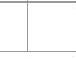
\includegraphics[max width=\textwidth]{2024_11_21_23d228cacd5e4a9a3f86g-08}
 &  &  \\
\hline
\end{tabular}
\end{center}

Zadanie 27. (2 pkt)\\
Wykaż, że liczba \(4^{23}+4^{22}-4^{21}\) jest podzielna przez 38.

\begin{center}
\begin{tabular}{|c|c|c|c|c|c|c|c|c|c|c|c|c|c|c|c|c|c|c|c|c|c|c|c|c|c|c|c|c|c|c|c|}
\hline
 &  &  &  &  &  &  &  &  &  &  &  &  &  &  &  &  &  &  &  &  &  &  &  &  &  &  &  &  &  &  &  \\
\hline
 &  &  &  &  &  &  &  &  &  &  &  &  &  &  &  &  &  &  &  &  &  &  &  &  &  &  &  &  &  &  &  \\
\hline
 &  &  &  &  &  &  &  &  &  &  &  &  &  &  &  &  &  &  &  &  &  &  &  &  &  &  &  &  &  &  &  \\
\hline
 &  &  &  &  &  &  &  &  &  &  &  &  &  &  &  &  &  &  &  &  &  &  &  &  &  &  &  &  &  &  &  \\
\hline
 &  &  &  &  &  &  &  &  &  &  &  &  &  &  &  &  &  &  &  &  &  &  &  &  &  &  &  &  &  &  &  \\
\hline
 &  &  &  &  &  &  &  &  &  &  &  &  &  &  &  &  &  &  &  &  &  &  &  &  &  &  &  &  &  &  &  \\
\hline
 &  &  &  &  &  &  &  &  &  &  &  &  &  &  &  &  &  &  &  &  &  &  &  &  &  &  &  &  &  &  &  \\
\hline
 &  &  &  &  &  &  &  &  &  &  &  &  &  &  &  &  &  &  &  &  &  &  &  &  &  &  &  &  &  &  &  \\
\hline
 &  &  &  &  &  &  &  &  &  &  &  &  &  &  &  &  &  &  &  &  &  &  &  &  &  &  &  &  &  &  &  \\
\hline
 &  &  &  &  &  &  &  &  &  &  &  &  &  &  &  &  &  &  &  &  &  &  &  &  &  &  &  &  &  &  &  \\
\hline
 &  &  &  &  &  &  &  &  &  &  &  &  &  &  &  &  &  &  &  &  &  &  &  &  &  &  &  &  &  &  &  \\
\hline
 &  &  &  &  &  &  &  &  &  &  &  &  &  &  &  &  &  &  &  &  &  &  &  &  &  &  &  &  &  &  &  \\
\hline
 &  &  &  &  &  &  &  &  &  &  &  &  &  &  &  &  &  &  &  &  &  &  &  &  &  &  &  &  &  &  &  \\
\hline
 &  &  &  &  &  &  &  &  &  &  &  &  &  &  &  &  &  &  &  &  &  &  &  &  &  &  &  &  &  &  &  \\
\hline
 &  &  &  &  &  &  &  &  &  &  &  &  &  &  &  &  &  &  &  &  &  &  &  &  &  &  &  &  &  &  &  \\
\hline
 &  &  &  &  &  &  &  &  &  &  &  &  &  &  &  &  &  &  &  &  &  &  &  &  &  &  &  &  &  &  &  \\
\hline
 &  &  &  &  &  &  &  &  &  &  &  &  &  &  &  &  &  &  &  &  &  &  &  &  &  &  &  &  &  &  &  \\
\hline
 &  &  &  &  &  &  &  &  &  &  &  &  &  &  &  &  &  &  &  &  &  &  &  &  &  &  &  &  &  &  &  \\
\hline
 &  &  &  &  &  &  &  &  &  &  &  &  &  &  &  &  &  &  &  &  &  &  &  &  &  &  &  &  &  &  &  \\
\hline
 &  &  &  &  &  &  &  &  &  &  &  &  &  &  &  &  &  &  &  &  &  &  &  &  &  &  &  &  &  &  &  \\
\hline
\end{tabular}
\end{center}

Zadanie 28. (2 pkt)\\
Początkowe ramię kąta \(\alpha\) pokrywa się z dodatnią półosią osi odciętych, a na końcowym ramieniu tego kąta leży punkt \(\mathrm{P}(-5 ; 12)\). Oblicz wartość wyrażenia: \(\operatorname{tg} \alpha+\frac{1}{\cos \alpha}\).\\

\includegraphics[max width=\textwidth, center]{2024_11_21_23d228cacd5e4a9a3f86g-09}

Zadanie 29. (2 pkt)\\
Wykaż, że w dowolnym trapezie suma długości podstaw jest mniejsza od sumy długości przekątnych.\\

\includegraphics[max width=\textwidth, center]{2024_11_21_23d228cacd5e4a9a3f86g-09(1)}

Zadanie 30. (2 pkt)\\
Cięciwa CD okręgu o środku O przecina średnicę AB tego okręgu w punkcie M (rysunek). Kąt środkowy oparty na łuku CB ma miarę \(46^{\circ}\), a \(\Varangle C M B\) ma miarę \(80^{\circ}\). Oblicz \(|\Varangle A C D|\).\\

\includegraphics[max width=\textwidth, center]{2024_11_21_23d228cacd5e4a9a3f86g-10}

Zadanie 31. (3 pkt)\\
Wyznacz iloczyn zbiorów rozwiązań nierówności: \(\frac{x-2}{2} \leq 3(x+8)\) oraz \(4(x-1)-(2 x+7)<3\).

\begin{center}
\begin{tabular}{|c|c|c|c|c|c|c|c|c|c|c|c|c|c|c|c|c|c|c|c|c|c|c|c|c|c|c|c|c|c|c|c|}
\hline
 &  &  &  &  &  &  &  &  &  &  &  &  &  &  &  &  &  &  &  &  &  &  &  &  &  &  &  &  &  &  &  \\
\hline
 &  &  &  &  &  &  &  &  &  &  &  &  &  &  &  &  &  &  &  &  &  &  &  &  &  &  &  &  &  &  &  \\
\hline
 &  &  &  &  &  &  &  &  &  &  &  &  &  &  &  &  &  &  &  &  &  &  &  &  &  &  &  &  &  &  &  \\
\hline
 &  &  &  &  &  &  &  &  &  &  &  &  &  &  &  &  &  &  &  &  &  &  &  &  &  &  &  &  &  &  &  \\
\hline
 &  &  &  &  &  &  &  &  &  &  &  &  &  &  &  &  &  &  &  &  &  &  &  &  &  &  &  &  &  &  &  \\
\hline
 &  &  &  &  &  &  &  &  &  &  &  &  &  &  &  &  &  &  &  &  &  &  &  &  &  &  &  &  &  &  &  \\
\hline
 &  &  &  &  &  &  &  &  &  &  &  &  &  &  &  &  &  &  &  &  &  &  &  &  &  &  &  &  &  &  &  \\
\hline
 &  &  &  &  &  &  &  &  &  &  &  &  &  &  &  &  &  &  &  &  &  &  &  &  &  &  &  &  &  &  &  \\
\hline
 &  &  &  &  &  &  &  &  &  &  &  &  &  &  &  &  &  &  &  &  &  &  &  &  &  &  &  &  &  &  &  \\
\hline
 &  &  &  &  &  &  &  &  &  &  &  &  &  &  &  &  &  &  &  &  &  &  &  &  &  &  &  &  &  &  &  \\
\hline
 &  &  &  &  &  &  &  &  &  &  &  &  &  &  &  &  &  &  &  &  &  &  &  &  &  &  &  &  &  &  &  \\
\hline
 &  &  &  &  &  &  &  &  &  &  &  &  &  &  &  &  &  &  &  &  &  &  &  &  &  &  &  &  &  &  &  \\
\hline
 &  &  &  &  &  &  &  &  &  &  &  &  &  &  &  &  &  &  &  &  &  &  &  &  &  &  &  &  &  &  &  \\
\hline
 &  &  &  &  &  &  &  &  &  &  &  &  &  &  &  &  &  &  &  &  &  &  &  &  &  &  &  &  &  &  &  \\
\hline
 &  &  &  &  &  &  &  &  &  &  &  &  &  &  &  &  &  &  &  &  &  &  &  &  &  &  &  &  &  &  &  \\
\hline
 &  &  &  &  &  &  &  &  &  &  &  &  &  &  &  &  &  &  &  &  &  &  &  &  &  &  &  &  &  &  &  \\
\hline
 &  &  &  &  &  &  &  &  &  &  &  &  &  &  &  &  &  &  &  &  &  &  &  &  &  &  &  &  &  &  &  \\
\hline
 &  &  &  &  &  &  &  &  &  &  &  &  &  &  &  &  &  &  &  &  &  &  &  &  &  &  &  &  &  &  &  \\
\hline
 &  &  &  &  &  &  &  &  &  &  &  &  &  &  &  &  &  &  &  &  &  &  &  &  &  &  &  &  &  &  &  \\
\hline
 &  &  &  &  &  &  &  &  &  &  &  &  &  &  &  &  &  &  &  &  &  &  &  &  &  &  &  &  &  &  &  \\
\hline
 &  &  &  &  &  &  &  &  &  &  &  &  &  &  &  &  &  &  &  &  &  &  &  &  &  &  &  &  &  &  &  \\
\hline
\end{tabular}
\end{center}

Zadanie 32. (4 pkt)\\
Poniżej przedstawiony jest wykres funkcji \(y=f(x)\). Na podstawie tego wykresu oblicz wartość wyrażenia \(3 \cdot f(2)-f(-4)\) oraz podaj:\\
a) dziedzinę funkcji \(f\),\\
b) maksymalne przedziały, w których funkcja \(f\) jest malejąca,\\
c) zbiór argumentów, dla których funkcja f przyjmuje wartości nieujemne.\\
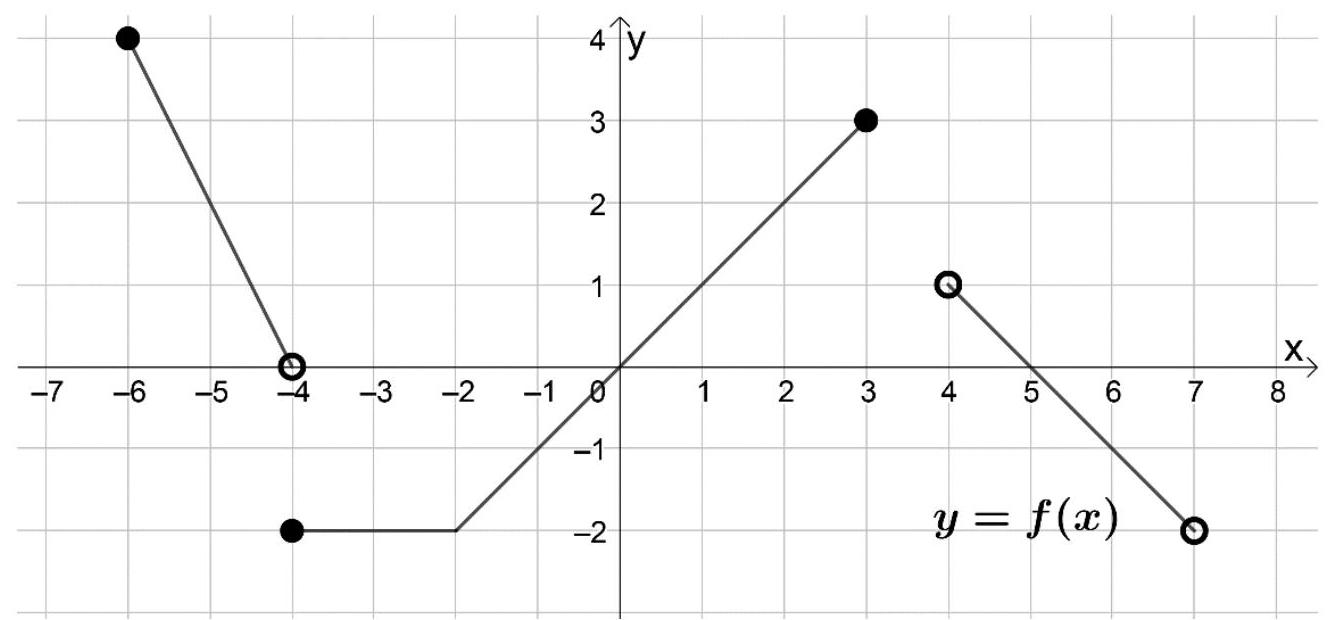
\includegraphics[max width=\textwidth, center]{2024_11_21_23d228cacd5e4a9a3f86g-11}

\begin{center}
\begin{tabular}{|c|c|c|c|c|c|c|c|c|c|c|c|c|c|c|c|c|c|c|c|c|c|c|c|c|c|c|c|c|c|c|c|}
\hline
 &  &  &  &  &  &  &  &  &  &  &  &  &  &  &  &  &  &  &  & \textbackslash  & 的 & ( & \textbackslash  & 的 & 的 & 的 &  &  &  &  &  \\
\hline
 &  &  &  &  &  &  &  &  &  &  &  &  &  &  &  &  &  &  &  &  &  &  &  &  &  &  &  &  &  &  &  \\
\hline
 &  &  &  &  &  &  &  &  &  &  &  &  &  &  &  &  &  &  &  &  &  &  &  &  &  &  &  &  &  &  &  \\
\hline
 &  &  &  &  &  &  &  &  &  &  &  &  &  &  &  &  &  &  &  &  &  &  &  &  &  &  &  &  &  &  &  \\
\hline
 &  &  &  &  &  &  &  &  &  &  &  &  &  &  &  &  &  &  &  &  &  &  &  &  &  &  &  &  &  &  &  \\
\hline
 &  &  &  &  &  &  &  &  &  &  &  &  &  &  &  &  &  &  &  &  &  &  &  &  &  &  &  &  &  &  &  \\
\hline
 &  &  &  &  &  &  &  &  &  &  &  &  &  &  &  &  &  &  &  &  &  &  &  &  &  &  &  &  &  &  &  \\
\hline
 &  &  &  &  &  &  &  &  &  &  &  &  &  &  &  &  &  &  &  &  &  &  &  &  &  &  &  &  &  &  &  \\
\hline
 &  &  &  &  &  &  &  &  &  &  &  &  &  &  &  &  &  &  &  &  &  &  &  &  &  &  &  &  &  &  &  \\
\hline
 &  &  &  &  &  &  &  &  &  &  &  &  &  &  &  &  &  &  &  &  &  &  &  &  &  &  &  &  &  &  &  \\
\hline
 &  &  &  &  &  &  &  &  &  &  &  &  &  &  &  &  &  &  &  &  &  &  &  &  &  &  &  &  &  &  &  \\
\hline
 &  &  &  &  &  &  &  &  &  &  &  &  &  &  &  &  &  &  &  &  &  &  &  &  &  &  &  &  &  &  &  \\
\hline
 &  &  &  &  &  &  &  &  &  &  &  &  &  &  &  &  &  &  &  &  &  &  &  &  &  &  &  &  &  &  &  \\
\hline
 &  &  &  &  &  &  &  &  &  &  &  &  &  &  &  &  &  &  &  &  &  &  &  &  &  &  &  &  &  &  &  \\
\hline
 &  &  &  &  &  &  &  &  &  &  &  &  &  &  &  &  &  &  &  &  &  &  &  &  &  &  &  &  &  &  &  \\
\hline
 &  &  &  &  &  &  &  &  &  &  &  &  &  &  &  &  &  &  &  &  &  &  &  &  &  &  &  &  &  &  &  \\
\hline
 &  &  &  &  &  &  &  &  &  &  &  &  &  &  &  &  &  &  &  &  &  &  &  &  &  &  &  &  &  &  &  \\
\hline
 &  &  &  &  &  &  &  &  &  &  &  &  &  &  &  &  &  &  &  &  &  &  &  &  &  &  &  &  &  &  &  \\
\hline
 &  &  &  &  &  &  &  &  &  &  &  &  &  &  &  &  &  &  &  &  &  &  &  &  &  &  &  &  &  &  &  \\
\hline
 &  &  &  &  &  &  &  &  &  &  &  &  &  &  &  &  &  &  &  &  &  &  &  &  &  &  &  &  &  &  &  \\
\hline
 &  &  &  &  &  &  &  &  &  &  &  &  &  &  &  &  &  &  &  &  &  &  &  &  &  &  &  &  &  &  &  \\
\hline
 &  &  &  &  &  &  &  &  &  &  &  &  &  &  &  &  &  &  &  &  &  &  &  &  &  &  &  &  &  &  &  \\
\hline
 &  &  &  &  &  &  &  &  &  &  &  &  &  &  &  &  &  &  &  &  &  &  &  &  &  &  &  &  &  &  &  \\
\hline
 &  &  &  &  &  &  &  &  &  &  &  &  &  &  &  &  &  &  &  &  &  &  &  &  &  &  &  &  &  &  &  \\
\hline
 &  &  &  &  &  &  &  &  &  &  &  &  &  &  &  &  &  &  &  &  &  &  &  &  &  &  &  &  &  &  &  \\
\hline
 &  &  &  &  &  &  &  &  &  &  &  &  &  &  &  &  &  &  &  &  &  &  &  &  &  &  &  &  &  &  &  \\
\hline
 &  &  &  &  &  &  &  &  &  &  &  &  &  &  &  &  &  &  &  &  &  &  &  &  &  &  &  &  &  &  &  \\
\hline
 &  &  &  &  &  &  &  &  &  &  &  &  &  &  &  &  &  &  &  &  &  &  &  &  &  &  &  &  &  &  &  \\
\hline
\end{tabular}
\end{center}

Zadanie 33. (4 pkt)\\
Dane są dwie liczby \(a\) i \(b\), których stosunek wynosi 4 : 5. Jeżeli mniejszą z tych liczb zwiększymy o \(25 \%\), a większą zmniejszymy o 40 , to stosunek otrzymanych liczb wyniesie \(3: 2\). Oblicz wartość wyrażenia: \(\frac{|a-b|}{\sqrt{30 b}}\).\\

\includegraphics[max width=\textwidth, center]{2024_11_21_23d228cacd5e4a9a3f86g-12}

Zadanie 34. (4 pkt)\\
Bok \(A B\) trójkąta \(A B C\) jest średnicą okręgu opisanego na tym trójkącie. Bok \(B C\) jest o 4 cm krótszy od boku \(A B\) oraz \(|A C|=8 \mathrm{~cm}\). Oblicz pole trójkąta \(A B C\) oraz długość promienia okręgu wpisanego w ten trójkąt.\\

\includegraphics[max width=\textwidth, center]{2024_11_21_23d228cacd5e4a9a3f86g-13}

\begin{center}
\begin{tabular}{|c|c|c|c|c|c|c|c|c|c|c|c|c|c|c|c|c|c|c|c|c|c|c|c|c|}
\hline
 &  &  &  &  &  &  &  &  &  &  &  &  &  &  &  &  &  &  &  &  &  &  &  &  \\
\hline
 &  &  &  &  &  &  &  &  &  &  &  &  &  &  &  &  &  &  &  &  &  &  &  &  \\
\hline
 &  &  &  &  &  &  &  &  &  &  &  &  &  &  &  &  &  &  &  &  &  &  &  &  \\
\hline
 &  &  &  &  &  &  &  &  &  &  &  &  &  &  &  &  &  &  &  &  &  &  &  &  \\
\hline
 &  &  &  &  &  &  &  &  &  &  &  &  &  &  &  &  &  &  &  &  &  &  &  &  \\
\hline
 &  &  &  &  &  &  &  &  &  &  &  &  &  &  &  &  &  &  &  &  &  &  &  &  \\
\hline
 &  &  &  &  &  &  &  &  &  &  &  &  &  &  &  &  &  &  &  &  &  &  &  &  \\
\hline
 &  &  &  &  &  &  &  &  &  &  &  &  &  &  &  &  &  &  &  &  &  &  &  &  \\
\hline
 &  &  &  &  &  &  &  &  &  &  &  &  &  &  &  &  &  &  &  &  &  &  &  &  \\
\hline
 &  &  &  &  &  &  &  &  &  &  &  &  &  &  &  &  &  &  &  &  &  &  &  &  \\
\hline
 &  &  &  &  &  &  &  &  &  &  &  &  &  &  &  &  &  &  &  &  &  &  &  &  \\
\hline
 &  &  &  &  &  &  &  &  &  &  &  &  &  &  &  &  &  &  &  &  &  &  &  &  \\
\hline
 &  &  &  &  &  &  &  &  &  &  &  &  &  &  &  &  &  &  &  &  &  &  &  &  \\
\hline
 &  &  &  &  &  &  &  &  &  &  &  &  &  &  &  &  &  &  &  &  &  &  &  &  \\
\hline
 &  &  &  &  &  &  &  &  &  &  &  &  &  &  &  &  &  &  &  &  &  &  &  &  \\
\hline
 &  &  &  &  &  &  &  &  &  &  &  &  &  &  &  &  &  &  &  &  &  &  &  &  \\
\hline
 &  &  &  &  &  &  &  &  &  &  &  &  &  &  &  &  &  &  &  &  &  &  &  &  \\
\hline
 &  &  &  &  &  &  &  &  &  &  &  &  &  &  &  &  &  &  &  &  &  &  &  &  \\
\hline
 &  &  &  &  &  &  &  &  &  &  &  &  &  &  &  &  &  &  &  &  &  &  &  &  \\
\hline
 &  &  &  &  &  &  &  &  &  &  &  &  &  &  &  &  &  &  &  &  &  &  &  &  \\
\hline
 &  &  &  &  &  &  &  &  &  &  &  &  &  &  &  &  &  &  &  &  &  &  &  &  \\
\hline
 &  &  &  &  &  &  &  &  &  &  &  &  &  &  &  &  &  &  &  &  &  &  &  &  \\
\hline
 &  &  &  &  &  &  &  &  &  &  &  &  &  &  &  &  &  &  &  &  &  &  &  &  \\
\hline
 &  &  &  &  &  &  &  &  &  &  &  &  &  &  &  &  &  &  &  &  &  &  &  &  \\
\hline
 &  &  &  &  &  &  &  &  &  &  &  &  &  &  &  &  &  &  &  &  &  &  &  &  \\
\hline
 &  &  &  &  &  &  &  &  &  &  &  &  &  &  &  &  &  &  &  &  &  &  &  &  \\
\hline
 &  &  &  &  &  &  &  &  &  &  &  &  &  &  &  &  &  &  &  &  &  &  &  &  \\
\hline
 &  &  &  &  &  &  &  &  &  &  &  &  &  &  &  &  &  &  &  &  &  &  &  &  \\
\hline
 &  &  &  &  &  &  &  &  &  &  &  &  &  &  &  &  &  &  &  &  &  &  &  &  \\
\hline
 & 唟 &  &  &  &  &  &  &  &  &  &  &  &  &  &  &  &  &  &  &  &  &  &  &  \\
\hline
 &  &  &  &  &  &  &  &  &  &  &  &  &  &  &  &  &  &  &  &  &  &  &  &  \\
\hline
 &  &  &  &  &  &  &  &  &  &  &  &  &  &  &  &  &  &  &  &  &  &  &  &  \\
\hline
 &  &  &  &  &  &  &  &  &  &  &  &  &  &  &  &  &  &  &  &  &  &  &  &  \\
\hline
 &  &  &  &  &  &  &  &  &  &  &  &  &  &  &  &  &  &  &  &  &  &  &  &  \\
\hline
 &  &  &  &  &  &  &  &  &  &  &  &  &  &  &  &  &  &  &  &  &  &  &  &  \\
\hline
 &  &  &  &  &  &  &  &  &  &  &  &  &  &  &  &  &  &  &  &  &  &  &  &  \\
\hline
 &  &  &  &  &  &  &  &  &  &  &  &  &  &  &  &  &  &  &  &  &  &  &  &  \\
\hline
 &  &  &  &  &  &  &  &  &  &  &  &  &  &  &  &  &  &  &  &  &  &  &  &  \\
\hline
 &  &  &  &  &  &  &  &  &  &  &  &  &  &  &  &  &  &  &  &  &  &  &  &  \\
\hline
 &  &  &  &  &  &  &  &  &  &  &  &  &  &  &  &  &  &  &  &  &  &  &  &  \\
\hline
 &  &  &  &  &  &  &  &  &  &  &  &  &  &  &  &  &  &  &  &  &  &  &  &  \\
\hline
 &  &  &  &  &  &  &  &  &  &  &  &  &  &  &  &  &  &  &  &  &  &  &  &  \\
\hline
 &  &  &  &  &  &  &  &  &  &  &  &  &  &  &  &  &  &  &  &  &  &  &  &  \\
\hline
 &  &  &  &  &  &  &  &  &  &  &  &  &  &  &  &  &  &  &  &  &  &  &  &  \\
\hline
 &  &  &  &  &  &  &  &  &  &  &  &  &  &  &  &  &  &  &  &  &  &  &  &  \\
\hline
 &  &  &  &  &  &  &  &  &  &  &  &  &  &  &  &  &  &  &  &  &  &  &  &  \\
\hline
 &  &  &  &  &  &  &  &  &  &  &  &  &  &  &  &  &  &  &  &  &  &  &  &  \\
\hline
 &  &  &  &  &  &  &  &  &  &  &  &  &  &  &  &  &  &  &  &  &  &  &  &  \\
\hline
 &  &  &  &  &  &  &  &  &  &  &  &  &  &  &  &  &  &  &  &  &  &  &  &  \\
\hline
\end{tabular}
\end{center}

\begin{center}
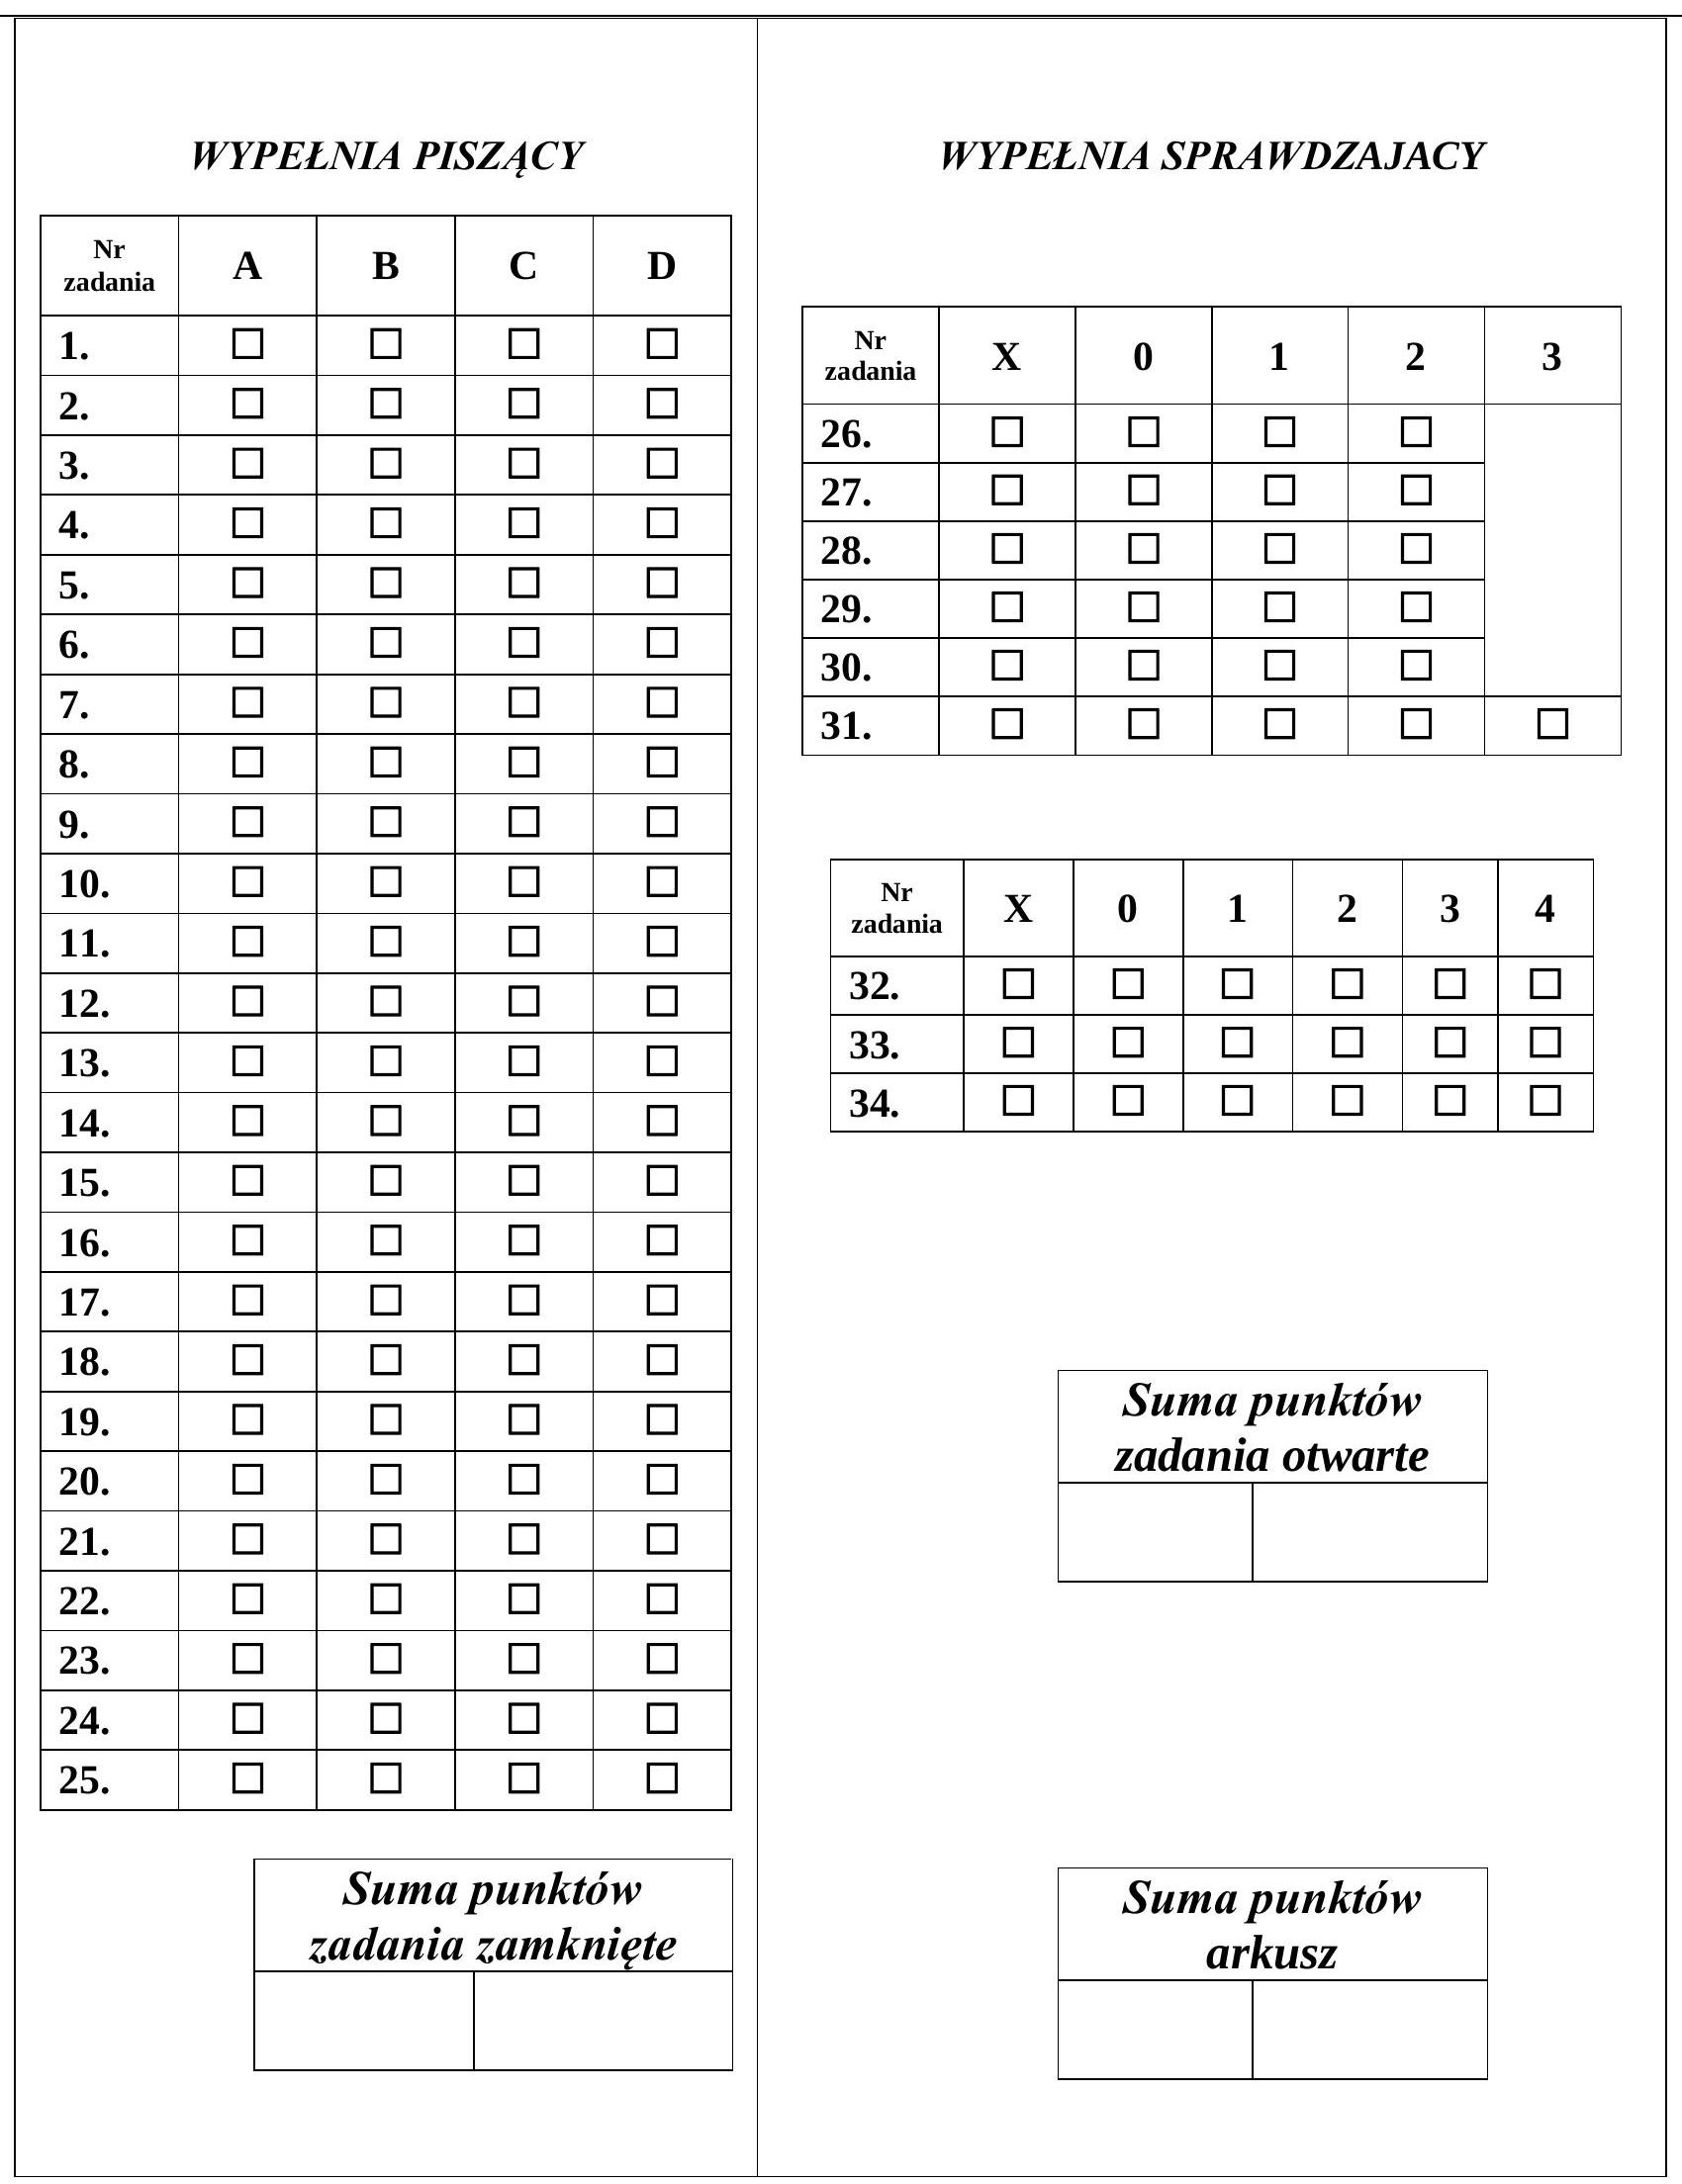
\includegraphics[max width=\textwidth]{2024_11_21_23d228cacd5e4a9a3f86g-16}
\end{center}


\end{document}